\documentclass[12pt,a4paper,bibtotoc]{scrartcl}

\usepackage[ngerman]{babel}
\usepackage[utf8]{inputenc}
\usepackage[T1]{fontenc}
\usepackage{csquotes}
\usepackage[pdftex]{graphicx}  

% Das Paket biblatex ist für Literaturverweise zuständig.
\usepackage[backend=biber,
            style=numeric
           ]{biblatex}
           
\graphicspath{{bilder/}}
           
\title{Planung und Erstellung einer Backend-Microservices-Architektur aus den Anforderungen durch das Spiel Stirnraten.}
\author{Michael Rothkegel}
\date{\today}

\addbibresource{literatur.bib}

\begin{document}

%
\maketitle
\tableofcontents
\newpage

%es gibt auch include - weiß den Unterschied noch nicht
%oder include only
\section{Einleitung}\label{sec:einleitung}

%Den Satz ggf umdrehen
Wenn ein Onlineshop genutzt wird, wirkt dieser wie eine einzelne Softwareanwendung. Es wird sich durch Artikel geklickt, der Warenkorb befüllt und schließlich eine Bestellung abgesendet. Wächst ein Onlineshop, wird dieser entsprechend komplexer und bietet zahlreiche Funktionalitäten. Auf Softwareebene entstehen dadurch Herausforderungen wie z.B. mit steigenden Benutzerzahlen oder vermehrten Datensätzen umgegangen wird. Dieses Phänomen betrifft natürlich nicht nur Onlineshops, sondern alle Softwareanwendungen, die viel genutzt werden, wie z.B. Spiele- oder Streamingplattformen, soziale Netzwerke, Buchungsseiten für Hotels, Auto oder Flüge usw. Zusätzlich entstehen innerhalb des Unternehmens Herausforderungen. An großer Software arbeiten in der Regel viele Mitarbeiter, diese müssen sich entsprechend organisieren und absprechen, damit sie nicht destruktiv arbeiten.\\

%Verweisen auf irgendwelche Quellen mit otto, google usw.
Abhilfe schafft die sogenannte Microservicesarchitektur. Die Idee ist eine große Softwareanwendung (Monolith) in viele kleine, eigenständig und in sich funktionierende Anwendungen (Microservices) zu zerteilen. Viele große Unternehmen wie Netflix, Amazon und Google bauen ihre Dienste bereits so auf. Aber auch deutsche Unternehmen wie Zalando, Otto oder Rewe nutzen bereits diese Art der Architektur. Die Anwendung für den Benutzer erscheint dabei komplett gleich.\\

Auf technischer Ebene bietet dies einfache Möglichkeiten der Skalierung, schnelle Updatezyklen und Agilität. Auch auf personeller Ebene kann die Organisation leichter werden, denn kleinere Teams sind verantwortlich für Microservices und können diesen entsprechend weiterentwickeln ohne andere Teams zu blockieren oder womöglich Fehler einzubauen. \\

%genauer noch drauf eingehen, Konzeption, implementierung, User Story Mappign
In der folgenden Arbeit wird eine API exemplarisch nach Microservice Gesichtspunkten erarbeitet. Dafür wird zunächst untersucht, inwiefern sich der Monolith zu den Microservices unterscheidet und wie man Microservices untereinander abgrenzen kann. Ebenfalls wird die Schnittstellenkommunikation zwischen Microservices beleuchtet sowie die Herausforderung einer Authentifizeriung und Autorisierung. Zusätzlich wird die Infrastruktur zum Aufsetzen (Docker) und die Erreichbarkeit (API-Gateway) behandelt.\\ 

Anschließend werden Anforderungen, die an die Stirnraten API gestellt werden, mittels User Story Mapping erfasst und herausgearbeitet. Für die Umsetzung werden in der Konzeption verschiedene Technologien und Strategien gegeneinander abgewogen und darauf beruhend in der Implementierung verwendet.\\ 

Ziel ist es eine lauffähige Stirnraten API basierend auf der Microservice Architektur umzusetzen und der App die Möglichkeit zur Kommunikation mit einem Backend zu geben. \\

\section{Grundlagen}

Der folgende Abschnitt arbeitet eine Abgrenzung zwischen einer Microservice- und monolithischen Architektur heraus. Zusätzlich geht er auf unterschiedliche Kommunikationsarten bei Microservices sowie die Authentifizierung und Autorisierung ein. 

\subsection{Definition Microservices}

Für den Begriff Microservices existiert keine einheitlich anerkannte Definition. Während Wolff unter Microservices unabhängige, deploybare Module versteht\cite{wolff2018mic_praxis}, spricht Newman von kleinen, autonomen Services, die zusammenarbeiten. Cockcroft verwendet den Begriff Microservice gekoppelt mit einem Architekturbegriff: Eine Microservice Architektur sind gekoppelte Services, welche für einen gewissen Kontextbereich zuständig sind.\cite{irakli2016mic_arc} D.h. jeder Service behandelt gewisse, fachliche Aufgaben und kann genau für diese genutzt werden. Eine Vielzahl von solchen Services bildet dann die gesamte Anwendung. \\

Amudsen schreibt dem Microservice an sich die Eigenschaft zu, dass er unabhängig zu anderen Microservices sein muss, d.h. ein Microservice kann losgelöst von anderen geupdated (deployed) werden. Weiter ist ein Microservice wie schon bei Cockcroft für einen gewissen Aufgabenbereich zuständig. Eine Microservice-Architektur ist ein zusammenschluss von miteinander kommunizierenden Microservices.\cite{irakli2016mic_arc} \\

In \textit{Flexible Software Architecture}\cite{wolff2016mic_architectures} werden Microservices zu den bisherigen Eigenschaften noch weitere, teils technische zugeschrieben: Microservices sind technologisch unabhängig, d.h. eine Microservice-Architektur ist beispielsweise nicht an eine bestimmte Programmiersprache oder Datenbank gebunden. Weiter müssen Microservices einen privaten Datenspeicher haben und sie kommunizieren mit anderen Services über das Netzwerk (z.B. über REST). Ebenfalls werden Microservices verwendet, um große Programme in kleine Teile zu unterteilen. Diese kleinen Teile lassen sich automatisch bauen und deployen. \\

Basierend auf den folgenden Definitionen wird der Microservice Begriff wie folgt verwendet: Microservices sind
\begin{itemize}
	\item klein in der Größe,
	\item kommunizieren mit anderen Services über Netzwerkschnittstellen (z.B. REST),
	\item sind unabhängig voneinander deploybar,
	\item können unabhängig voneinander entwickelt werden (d.h. Microservice A muss nicht auf B,C,D … warten und/oder umgekehrt),    
	\item eingeschränkt in ihrer Geschäftslogik, d.h. ein Microservice kümmert sich immer um einen speziellen Kontext, der im Vorhinein definiert werden muss,
	\item dezentral, d.h. sie können auf unterschiedlichsten Plattformen gehosted werden.
\end{itemize}

Abschließend handelt es sich um eine Microservice-Architektur, wenn viele Microservices nach Definition verwendet werden. 

\subsection{Monolithische Struktur }

Eine monolithische Struktur ist ein einziges Softwareprogramm (Monolith), welches in sich geschlossen ist. Dies bedeutet im Detail, dass ein Monolith aus mehreren Ebenen besteht, auf die über Schnittstellen zugegriffen werden kann. Innerhalb der Ebenen werden Komponenten wie z.B. Frameworks oder selbstgeschriebene Klassen eingebunden und verwendet.\cite{msfussell2017azure} Durch die sich aufeinander aufbauenden Ebenen folgt daraus, dass sämtliche Geschäftslogiken, User Interfaces sowie die Datenbank und Datenbankzugriffe Abhängigkeiten haben. All dies ist in einem Programm vereint.\cite{msfussell2017azure} Natürlich kann die monolithische Struktur innerhalb noch einmal Modular sein, d.h. in einem Monolithen existierten ggf. mehrere Module, welche verschiedene Geschäftslogiken abbilden. Dennoch können diese Module nicht unabhängig von der gesamten Anwendung deployed werden.\cite{nhiem2017mic_moving}

\begin{figure}[ht]
	\centering
	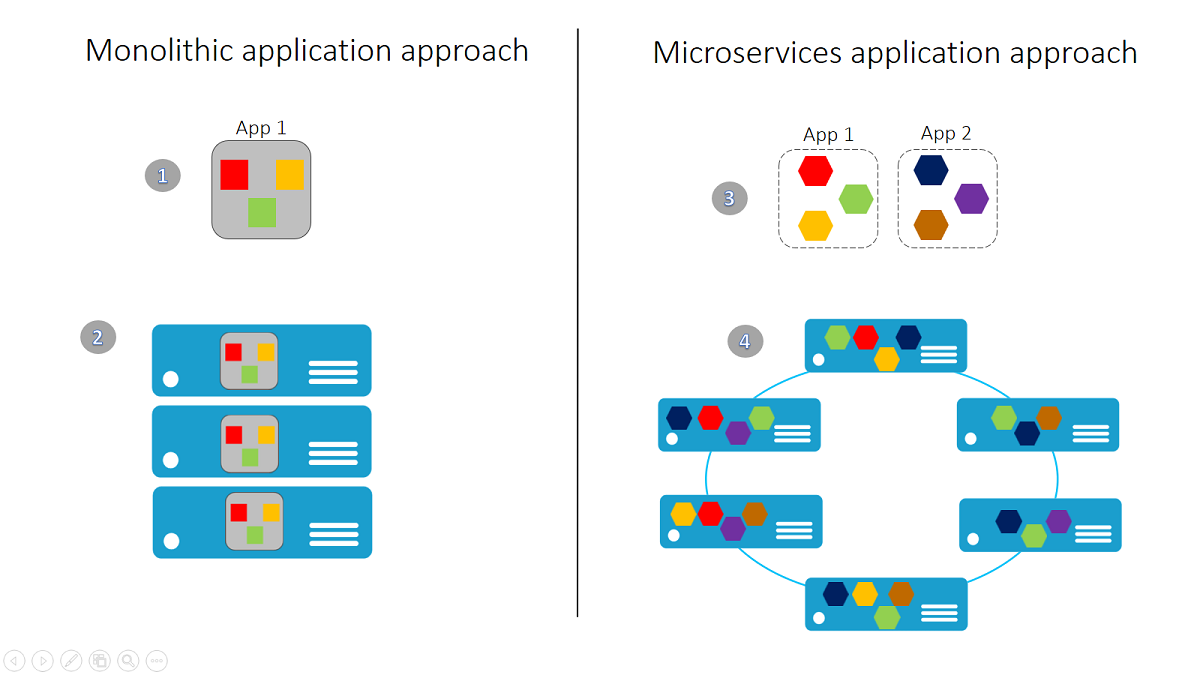
\includegraphics[width=0.9\textwidth]{monolithic_vs_micro}
	\caption[Monolith und Microservice-Architektur] {Monolith und Microservice-Architektur.\cite{msfussell2017azure}}
	\label{fig:mono}
\end{figure}

Abbildung \ref{fig:mono} zeigt eine vereinfachte Gegenüberstellung der beiden Architekturen. Die App 1 ist in drei klassische Funktionen (Web, Business und Data) unterteilt. Die Skalierung (2) kann durchgeführt werden, indem App 1 über mehrere Server oder VMs geklont wird. 

Bei der Microservice-Architektur werden die Funktionen auf unterschiedliche Dienste aufgeteilt. Konkreter könnte dies bedeuten, dass App 1 bei (3) zuständig für eine Benutzerkontoverwaltung ist und App 2 für ein Abrechnungssystem. Die Microservices (4) werden nicht geklont, sondern können unabhängig voneinander bereitgestellt werden. 

\subsection{Monolith vs. Microservices}\label{sec:monolith_vs_microservices}
Aus den vorherigen Abschnitten sind diverse Unterschiede zwischen den Architekturen erkennbar geworden. Nun gilt es festzustellen, welche Architekturen für welche Problemstellungen, sinnvoller ist. \cite{wolff2016mic_architectures} \cite{birk2016mic_soa}
%TODO: Nicht sicher, wo \cite{wolff2016mic_architectures} \cite{birk2016mic_soa} und genau platziert werden sollten
\begin{table}
	\begin{center}
		\begin{tabular}{|p{4cm}|p{5cm}|p{5cm}|}
			& Monolithische Architektur & Microservice-Architektur \\ \hline
			Abhängigkeiten & all1es in einer Anwendung & entkoppelt, da Prinzip von Modularisierung verwendet wird \\  \hline
			Größe & linear steigend & einzelne Services sind klein \\  \hline
			\raggedright{Geschwindigkeit der Zugriffe} & schnell, da alles in einer Anwendung & Zugriffe können länger dauern \\  \hline
			Deployment & schwieriger je größer das Projekt, aufgrund von
			\begin{itemize}
				\item Abhängigkeiten  
				\item Größe \end{itemize}
			 & einfach, da Microservices \begin{itemize}
				\item klein und 
			    \item modular sind \end{itemize} \\  \hline
			Organisation & leichter, da alles an einem Ort & schwerer, da mehr Domänenlogik (wer macht was?) beachtet werden muss \\  \hline
			Legacy-Systeme ablösen & ggf. schwierig, da System sehr verzahnt mit anderen Technologien ist & leicht, da Microservices durch neue abgelöst werden können \\  \hline
			Technologie & beschränkt & vielfältig \\  \hline
			Nachhaltige Entwicklung & wartbar mit Einschränkungen & leicht wartbar \\  \hline
			Robustheit & weniger, da ganzes System bei schweren Fehlern abstürzt & sehr, da im Zweifel immer nur ein Service abstürzt \\  \hline
			Skalierung & \raggedright{horizontale und vertikale Skalierung, Umsetzung kann sehr komplex werden} &  horizontale und vertikale Skalierung \\  \hline
			Betrieb & nur ein System & komplex, da mehr Services verwaltet werden müssen  \\ \hline
		\end{tabular} 
	\end{center}
	\caption[Monolitih vs. Mircoservice-Architektur]{Monolitih vs. Mircoservice-Architektur}
	\label{tab:mono_vs_microservices} 
\end{table}

Aus der Tabelle \ref{tab:mono_vs_microservices} ergeben sich verschiedene Punkte: Der Monolith eignet sich besonders dann sehr gut, wenn die Projekt- sowie Teamgrößen absehbar und auch die benötigten Technologien klar sind. Zusätzlich kann ein Monolith beim Projektanfang von Vorteil sein, da die Abhängigkeiten innerhalb des Projektes liegen und so die Entwicklungsgeschwindigkeit nicht durch eine kompliziertere Infrastruktur blockiert wird. \\

Ist die Projektgröße allerdings nicht absehbar, treten früher oder später mehrere Schwierigkeiten auf: Zum einen bindet der am Anfang des Projektes festgelegte Technologiestack, d.h. die Nutzung oder der Austausch neuer Technologien ist in der Regel mit sehr viel Arbeit verbunden. Zum anderen führen die anfangs eingegangen Abhängigkeiten zu Problemen im Deployment (A kann erst updaten, wenn B soweit ist) und einem erhöhten Aufwand in der Kommunikation zwischen den Teams (A kann erst beginnen, wenn B xy erledigt hat). \\

Die Skalierung von Microservices dagegen ist unabhängiger. Es können sich feingranular Services gesucht werden, welche skaliert werden sollen. Diese benötigen nicht zwingend mehr Hardware (vertikale Skalierung), sondern könnten z.B. auch auf verschiedene Server verteilt werden (horizontale Skalierung). Dies ist bei einem Monolithen natürlich auch möglich, dennoch muss immer der ganze Monolith skaliert werden, welcher zum einen immer mehr Hardware als einzelne Microservices benötigt und zum anderen in der Regel auch durch die Komplexität schwerer zu skalieren ist.\cite{wolff2018mic_praxis}\\

Als abschließender Punkt ist die Robustheit zu erwähnen: Wenn ein Microservice einen Fehler enthält, stürzt dieser im schlechtesten Fall ab. Im besten Fall übernimmt dieser Service eine weniger wichtige Funktion und der Nutzer bemerkt den Ausfall noch nicht einmal. Beim Monolithen dagegen stürzt die gesamte Anwendungen ab. In der Regel startet so eine Anwendung automatisch neu, jedoch betrifft die Downtime alle Nutzer. \\

Eine generelle Aussage, welche Architektur besser oder schlecht ist, lässt sich dementsprechend nicht treffen. Es kommt immer darauf an, welche Zielsetzung und wie viele Ressourcen für das Projekt festgelegt sind. Eine monolithische Architektur ist schneller umsetzbar und es ist nicht gegeben, dass ein Softwareprodukt überhaupt so viel Nachfrage erzeugt und somit eine Microservice-Architektur notwendig ist. Dementsprechend muss abgewogen werden, welche Architektur für welchen Anwendungsfall besser geeignet ist.\cite{wolff2018mic_praxis} REWE Digital beispielsweise hat ihr Produkt zuerst als Monolithen gestartet und ist erst später auf eine Microservice-Architektur umgeschwenkt.\cite{rewe2019mic_ppp} 

\subsection{Architektur von Micrsoservices}

Wie bereits erwähnt, ist die Entkopplung von Microservices ein großer Vorteil gegenüber dem Monolithen. Dennoch ist es sinnvoll, Richtlinien, Regeln und/oder Festlegungen zu schaffen, damit die Microservices nicht blockierend oder technologisch gegensätzlich arbeiten. Die Entscheidungsebene kann global (Makroarchitektur) oder nur für einen einzelnen Service (Mikroarchitektur) gelten.\cite{wolff2016mic_architectures} Welche Festlegungen und mit welcher Strenge diese eingehalten werden müssen, hängt von verschiedenen Faktoren ab, welche technologisch, organisatorisch oder wirtschaftlich motiviert sein können.\cite{rewe2019mic_ppp} \\ 

In dem folgenden Abschnitt wird das Grundprinzip der Software-Modellierungs-Methodik Domain Driven Design untersucht. Zusätzlich wird erläutert, welche Fälle makro- oder microarchitektonisch einzuordnen sind. \\

\subsubsection{Domain Driven Design}\label{sec:domain_driven_design}

Domain Driven Design (DDD) ist ein Vorgehen, mit dem ein Softwaresystem modelliert werden kann. Im Sinne einer Microservice-Architektur kann dies als Werkzeug genutzt werden, um Microservices fachlich einzuteilen.\cite{heise2016ddd} Beim sogenannten \textit{Strategic Design} wird dafür das Softwaressytem in verschiedene \textit{Bounded Contexts} eingeteilt, welche an ein \textit{Domänenmodell} gebunden sind. Ein Domänenmodell bildet die Geschäftslogik ab, d.h. inwiefern einzelne Objekte innerhalb des Kontextes in Relation zueinander stehen, welche Eigenschaften sie haben und wie sie sich verhalten. Dabei kann ein Domänenmodell - je nach Entwurfsmuster - von einem oder mehreren Bounded Contexts genutzt werden.\cite{wolff2018mic_praxis}  \\

\begin{figure}[ht]
	\centering
	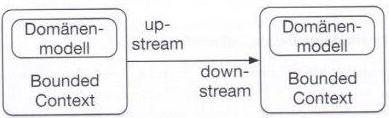
\includegraphics[width=0.5\textwidth]{bounded_context_1}
	\caption[Bounded Contexts mit eigenständigem Domänenmodel] {Bounded Contexts mit eigenständigem Domänenmodell.\cite{wolff2018mic_praxis}}
	\label{fig:bounded_context_with_own_datamodels}
\end{figure}

\begin{figure}[ht]
	\centering
	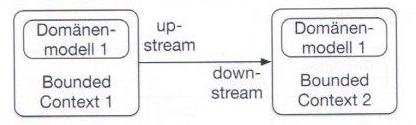
\includegraphics[width=0.5\textwidth]{bounded_context_2}
	\caption[Bounded Context 2 adaptiert das Domänenmodel von Bounded Context 1] {Bounded Context 2 adaptiert das Domänenmodel von Bounded Context 1.\cite{wolff2018mic_praxis}}
	\label{fig:bounded_context_with_copied_datamodel}
\end{figure}

\begin{figure}[ht]
	\centering
	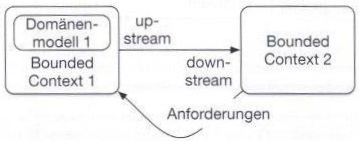
\includegraphics[width=0.5\textwidth]{bounded_context_3}
	\caption[Bounded Context 2 erhält ein auf ihn zugeschnittenes Domänenmodel von Bounded Context 1] {Bounded Context 2 erhält ein auf ihn zugeschnittenes Domänenmodel von Bounded Context 1.\cite{wolff2018mic_praxis}}
	\label{fig:bounded_context_with_custom_datamodels}
\end{figure}

Wolff verdeutlicht das Prinzip von Bounded Contexts mit Hilfe von vier Microservices, welche einen Onlineshop repräsentieren: \textit{Suche}, \textit{Check Out}, \textit{Inkasso} und \textit{Lieferung}. Während das Datenmodell der Suche detaillierte Informationen über die Produkte enthält, reicht es im Warenkorb (hier Check Out), wenn ggf. nur der Produktname gespeichert wird. Bei Inkasso ist es ähnlich: An dieser Stelle sind Zahlungsdaten des Benutzers relevant, während bei der Lieferung ggf. nur die Adresse notwendig ist.\cite{wolff2018mic_praxis} An diesem Beispiel wird deutlich, dass zwar von denselben Begrifflichkeiten wie Benutzer, Produkt usw. gesprochen wird, allerdings jeder Service sein eigenes Domänenmodell hat. Diese Technik ist unterstützend dabei, eine saubere Microservice-Architecktur abzubilden.\cite{wolff2018mic_praxis} \cite{heise2016ddd} \\

Neben der fachlichen Trennung bildet DDD auch die Kommunikation zwischen Kontexten ab. Dabei wird grundsätzlich vom \textit{up-stream} (vorgeschaltet) und dem \textit{down-stream} (nachgeschaltet) gesprochen.\cite{wolff2018mic_praxis} Der up-stream stellt dem down-stream Informationen bereit. Wie dies technisch umgesetzt ist, also ob der down-stream nachfragt oder der up-stream aktiv Daten schickt, ist frei wählbar. \\

Nach dem Anwenden von DDD sollte die Struktur der Software erkennbar sein: D.h. welche Art Microservices werden benötigt und inwiefern steht sie mit anderen in Abhängigkeiten oder in einer Kommunikation.   

\subsubsection{Macro- und Mikroarchitektur}\label{sec:macro_und_mikroarchitektur}

Wenn durch das DDD entworfen wird, welche Microservices voraussichtlich benötigt werden, ist es sinnvoll, einen Art Bauplan zu verfassen, welcher impliziert, an welche Regeln sich ein Microservice halten muss. Diese Regeln können wie bereits erwähnt auf globaler Ebene getroffen werden, d.h. sie gelten für alle Services (Makroarchitektur) oder sie gelten nur im Microservice selber (Microarchitektur). REWE Digital unterscheidet dabei zwischen \textit{Must}, \textit{Should}, \textit{Could}. D.h. es gibt Regeln, die Microservices erfüllen müssen, wie z.B. das Kommunzieren über REST oder das Implementieren einer einheitlichen Autorisierung.\cite{rewe2019mic_ppp} Andere Regeln dagegen sind viel mehr Richtlinien (should) oder komplett optional (could). Das Ziel ist stets, dass durch die makroarchitektonischen Entscheidungen nicht die Vorteile von Microservices beschnitten werden.\cite{wolff2018mic_praxis}\cite{irakli2016mic_arc}. \\

Es gibt verschiedene Einflussfaktoren wie sich die Makroarchitektur für ein Unternehmen definiert: Zum einen empfiehlt es sich, ein Gremium zu gründen, welches sich stetig mit den Regeln der Makroarchitektur auseinandersetzt, sie entsprechend erweitert, überarbeitet und die getroffenen Entscheidungen auch immer begründen kann.\cite{wolff2018mic_praxis} Zum anderen besteht immer ein technischer Einfluss\cite{wolff2018mic_praxis}:
\begin{itemize}
	\item Gewählte Technologien müssen in die Infrastruktur des Unternehmens passen: Angenommen die Auslastung eines Microservices muss überwacht werden und dies wird firmenweit mit Tool A erledigt, dann wäre es sehr aufwendig, wenn der besagte Service nur eine Schnittstelle für Tool B anbietet und der nächste Service nur für Tool C. Dies würde einerseits sehr unübersichtlich werden und andererseits viel Aufwand bedeuten. 
	\item Technologien sind immer von dem Personal abhängig: Gerade wenn Unternehmen klein bis mittelständig sind, empfiehlt es sich, Technologien zu nutzen, die mehrere Entwickler beherrschen, um Inselwissen zu reduzieren. 
	\item Ebenfalls können gezielt strategische Entscheidungen getroffen werden, z.B. wenn ein Unternehmen die Dateninfrastruktur zu einem Cloudanbieter auslagern möchte, hat dies entsprechende makroarchitekonische Auswirkungen.
\end{itemize}

Basierend auf Wolff und Nadareishvili ist Tabelle \ref{tab:macro_micro} entstanden, welche einen Überblick darüber gibt, wie gängige Themen eingeordnet werden können. \cite{wolff2018mic_praxis}\cite{irakli2016mic_arc}\cite{rewe2019mic_ppp}

\begin{table}[ht]
	\begin{center}
		\begin{tabular}{|p{5cm}|p{5cm}|p{5cm}|}
			& Mikroarchitektur & Makroarchitektur \\ \hline
			Programmiersprache &  x & x  \\ \hline
			Datenbank & x & x \\ \hline
			Look and Feel (UI) & x  & x  \\ \hline
			Dokumentation & x & x  \\ \hline
			Datenformat &   & x \\ \hline
			Kommunikationsprotokoll &   & x \\ \hline
			Authentifizierung &  & x \\ \hline
			Integrationtests &  &  x \\ \hline
			Autorisierung & x  &  \\ \hline
			Unittests & x  &  \\ \hline
			Continuous-Delivery-Pipeline & x &  \\ \hline
		\end{tabular}
	\end{center}
	\caption[Entscheidungen Micro- und Macroarchitektur]{Entscheidungen Micro- und Macroarchitektur}
	\label{tab:macro_micro} 
\end{table}

In der Tabelle \ref{tab:macro_micro} sieht man, dass gerade die ersten Punkten sehr von der Unternehmenskultur und den technischen sowie personellen Freiheiten abhängen. In der Theorie sollte die Programmiersprache sinnvoll für jeden Microservices gewählt werden, dennoch ergibt es auch Sinn, einen Pool an Programmiersprachen auf Makroebene zu definieren, um Inselwissen zu reduzieren und nachhaltige Codequalität zu gewährleisten. Ähnliches gilt beispielsweise für die Wahl der Datenbank: Ist bereits eine globale Infrastruktur für Datenbank X geschaffen, sollte diese nicht ohne Weiteres aufgebrochen werden, nur weil es technisch möglich ist. \\

Bei der Dokumentation sowie beim Look \& Feel ist es sinnvoll, globale Richtlinien zu definieren, damit klar ist, wo bei jedem Microservices die Dokumentation zu finden ist oder wie ein User Interface grundsätzlich angeordnet und gestaltet werden soll. Dennoch können diese Punkte im Detail je nach Microservice abweichen. \\

Ein Kommunikationsprotokoll (z.B. REST) sowie Datenformate (z.B. JSON) sollten festgeschrieben werden.\cite{rewe2019mic_ppp} \cite{wolff2018mic_praxis} Als Grund wird zum einen das Vermeiden von technischem Mehraufwand angegeben, zum anderen sind Microservices zwar eigenständig deploybare Einheiten, dennoch sollten sie technisch zum Gesamtsystem passen und nicht dagegen arbeiten. \\

Während die Authentifzierung (um wen handelt es sich) einmalig festgelegt werden sollte, liegt die Überprüfung der Autorisierung (was darf der Benutzer) in jedem Microservice selbst. Die Alternative wäre, dass jede eingehende Anfrage noch einmal geprüft wird, was zu unnötig hohem Traffic und somit zu Verzögerungen führen würde.  \\

Die hier erarbeitete Tabelle  \ref{tab:macro_micro}  ist an dieser Stelle nicht als feststehendes Manifest für alle Unternehmen zu verstehen, sondern zeigt eine mögliche, sinnvolle Einordnung. Natürlich können architektonische Entscheidungen stark vom jeweiligen Anwendungszweck abhängen. Nicht aufgeführt ist beispielsweise der Umgang mit Konfigurationsdateien, Monitoring oder Logging. Beim Monitoring könnte zum Beispiel global entschieden werden, \textit{wo} Metriken abgelegt werden bzw. mit \textit{welcher} Technologie gearbeitet wird. Aus microarchitektonischer Sicht könnten die Services allerdings selbst entscheiden, \textit{was} gemessen wird.  \\

Ebenso beim Deployment: Es gibt zahlreiche Methoden, um neue Updates bereitzustellen wie z.B. mittels Docker, Kubernetes oder indivudelle Installationsskripte.\cite{wolff2018mic_praxis} Welche Technologie sich durchsetzt, muss anhand der Anforderung entschieden werden. \\

Aus den erarbeitenten Punkten lassen sich Vor- und Nachteile ableiten. Vorteile für microarchitektonische Entscheidungen sind ein sehr hohes Maß an Flexibilität und eine hohe Unabhängigkeit im Gesamtsystem, was grundsätzlich das Ziel von Microservices ist. Dies wiederum kann dazu führen, dass Entwicklungsoverhead oder Inselwissen entsteht. Ebenfalls könnten Punkte wie z.B. das \textit{Look \& Feel} oder die \textit{Dokumentation} darunter leiden.  \\

Macroarchitektonische Entscheidungen haben zum Vorteil, dass es Regeln gibt, welche die Entwicklung vereinfachen sollen und gegebenfalls die Nachteile der Microarchitektur kompensieren können. Auf der anderen Seite schränken macroarchitekonische Entscheidungen ein. Zusätzlich müssen sie organisch, z.B durch ein extra dafür geschaffenes Gremium, durchgesetzt werden.\cite{wolff2018mic_praxis} Im Gesamten lässt sich daraus schließen, dass sehr genau abgewogen werden muss, welche Entscheidungen global oder individuell entschieden werden. Grundsätzlich gilt, dass jede Entscheidung begründbar sein muss.    

\subsection{Kommunikation}

Bei einem Monolithen wird eine Abfrage über eine Route gestellt, woraufhin die Anwendung entsprechend mit der Bearbeitung beginnt. Da die gesamte Datenhaltung an einer Stelle ist, sind alle Daten bekannt und abrufbar. Wichtiger noch: Die Daten sind konsistent. \\

Microservices sind diesbezüglich herausfordernder. Es müssen verschiedene architektonische Entscheidungen getroffen werden, wie z.B. ob es einen zentralen Service gibt, welcher alle Anfragen weiterleitet (\textbf{API Gateway}) oder ob jeder Service einzeln erreichbar ist. Ebenfalls sollte auch begründbar entschieden werden, ob eine synchrone,  asynchrone oder möglicherweise eine hybride Kommunikation verwendet wird. 

In den folgenden Unterkapiteln werden Vor- und Nachteile der verschiedenen Kommunikationsarten für Microservices mit einem Schwerpunkt auf Unabhängigkeit (Entkopplung) und Datenkonsistenz untersucht.

% Problem beschreiben, warum kann man nicht einfach alles über REST klären
% Beispiel aus Microservice in Action: Zwei Aufrufe gehen gut, der dritte nicht, ungewollten State.
% ggf. das 2PC Protokoll bemerken, dass das eine Lösung ist, aber auch nicht funktioniert: Gegengründe aufführen
%was ist die Lösung: Event Based

\subsubsection{Synchrone Kommunikation}\label{sec:synchrone_kommunikation}

Wenn ein Microservice bei der Bearbeitung einer Anfrage selbst eine weitere Anfrage an einen anderen Microservice stellen muss und auf das Ergebnis wartet, spricht man von synchroner Kommunikation.\cite{wolff2018mic_praxis} 

Anhand dieser Definition lässt sich folgendes Szenario darstellen (siehe Abbildung \ref{fig:synchrone_kommunikation_microservices}). 

\begin{figure}[ht]
	\centering
	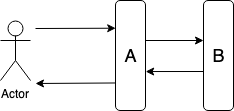
\includegraphics[width=0.5\textwidth]{synchrone_kommunikation_microservices}
	\caption[Synchrone Kommunikation] { Synchrone Kommunikation}
	\label{fig:synchrone_kommunikation_microservices}
\end{figure}

Der Actor stellt bei Microservice A eine Anfrage, welche bearbeitet und schließlich an B weiterleitet wird. B verarbeitet diese ebenfalls und antwortet, so dass auch A wieder antworten kann. Aus diesem Ablauf lässt sich festhalten, dass die übertragenden Daten aktuell sind. D.h. der Actor erhält definitiv konsistente Daten, was positiv zu vermerken ist. Problematischer dagegen ist die Abhängigkeit, welche entsteht. Sollte B nicht erreichbar sein, läuft A in einen Timeout und ist blockiert. Einerseits ließe sich argumentieren, dass genau dies passieren soll, schließlich scheint es einen Fehler zu geben. Aber angenommen A wäre ein Service zum Erstellen von Rechnungen und B ein Service zum Sammeln von Daten für Marktanalysen. A möchte B infomieren, dass eine neue Rechnung erstellt wurde, läuft allerdings in einen Timeout. Die Operation, eine Rechnung zu erstellen, hat allerdings eine höhere Priorität als es statistisch zu erfassen. Nach den aufgestellen Definitionen aus Abschnitt \ref{sec:monolith_vs_microservices} für Microservices wird die Entkopplung, Modularität und Robustheit des Systems verletzt, da A nicht weiterarbeiten kann.\cite{wolff2018mic_praxis} \cite{bruce2019mic_in_action}  

Bläht man das Beispiel auf, so dass weitere Services statistische Daten erfassen wollen, würden zahlreiche Microservices ausfallen (siehe Abbildung \ref{fig:snyn_com_dependencies}). \\

\begin{figure}[ht]
	\centering
	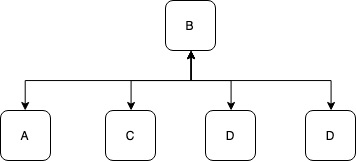
\includegraphics[width=0.5\textwidth]{snyn_com_dependencies}
	\caption[Abhängigkeiten in synchroner Kommunikation] { Abhängigkeiten in synchroner Kommunikation}
	\label{fig:snyn_com_dependencies}
\end{figure}

Die Microservices können auch nicht auf eine Notfallstrategie (\textbf{Fallback}) zurückgreifen. Nehme man an, Service B ist nach x Sekunden nicht erreichbar, so wird die ursprüngliche Abfrage durch A weiter abgearbeitet, um nicht zu blockieren. Nun müsste allerdings eine andere Logik dafür sorgen, dass die Daten, die nicht übertragen werden konnten, zu einem anderen Zeitpunkt nachgetragen werden. In diesem Moment würde keine Datenkonsistenz mehr gewährleistet sein. \\

Auch nicht zu vernachlässigen, ist die Geschwindigkeit, mit der die Abfragen abgearbeitet werden können. Möglicherweise muss B in einem anderen Szenario noch mit C kommunizieren. Die Anfrage würde sich über drei Services erstrecken, was zusätzliche Latenz mit sich bringt.\cite{wolff2018mic_praxis} \\   

Ebenfalls entsteht durch jede Schnittstelle eine fachliche Abhängigkeit.\cite{bruce2019mic_in_action} Die Anfragen von den Microservices A, C, D, E müssen der Schnittstellendefinition von B entsprechen. Änderungen führen gegebenenfalls zu Fehlern und weiteren Abhängigkeiten. Wie diese Problematik gelöst werden könnte, wird in Abschnitt \ref{sec:asynchrone_kommunikation} beschrieben.

\subsubsection{Asynchrone Kommunikation}\label{sec:asynchrone_kommunikation}

Wie bereits beschrieben, wird bei der synchronen Kommunikation auf weiterführende Abfragen gewartet. Die asynchrone Kommunikation wartet nicht auf Antworten von weiteren Services, sondern trifft Annahmen über etwaige Systemzustände.\cite{wolff2018mic_praxis} Um Annahmen zu treffen, existieren je nach Anwendungsfall verschiedene Strategien:

\begin{enumerate}
\item{ Ein Microservice kann replizierte Daten vorhalten. Angenommen ein Artikel soll rausgeschickt werden: Der dafür verantwortliche Service benötigt die Anschrift des Kunden, aber nicht weitere Daten wie Geburtsdatum, Zahlungsmethode oder ähnliches. Dementsprechend werden nur relevante Daten repliziert vorgehalten. Eine Herausforderung ist es, dass diese replizierten Daten stets mit den Originaldaten übereinstimmen. Schließlich kann sich eine Anschrift ändern.\cite{wolff2018mic_praxis}}

\item{Ggf. muss nur ein weiterer Service informiert werden, wie der Service B aus Abschnitt \ref{sec:synchrone_kommunikation}, welcher Statistiken erfasst. In dem Szenario der asynchronen Kommunikation würde die Abfrage gestellt werden, ohne das Ergebnis abzuwarten, da es schlichtweg nicht relevant ist. Die Herausforderung hier ist, zu gewährleisten, dass die Abfrage auch in Fehlerfällen früher oder später zugestellt wird.}
\end{enumerate}

Aus den Strategien ergeben sich Anforderungen an die Kommunikationsstruktur: Es muss gewährleisten sein, dass fehlerhafte Abfragen erneut übermittelt werden und ebenfalls wird eine Struktur benötigt, die dafür sorgt, dass replizierte Datensätze stets mit aktuellen Daten befüllt sind. Dies lässt sich durch sogenannte Events erreichen.\cite{bruce2019mic_in_action}\cite{wolff2018mic_praxis}  \\

Die folgende Abbildung \ref{fig:microservices_bus} verdeutlich das Prinzip von Events und deren Infrastruktur.

\begin{figure}[ht]
	\centering
	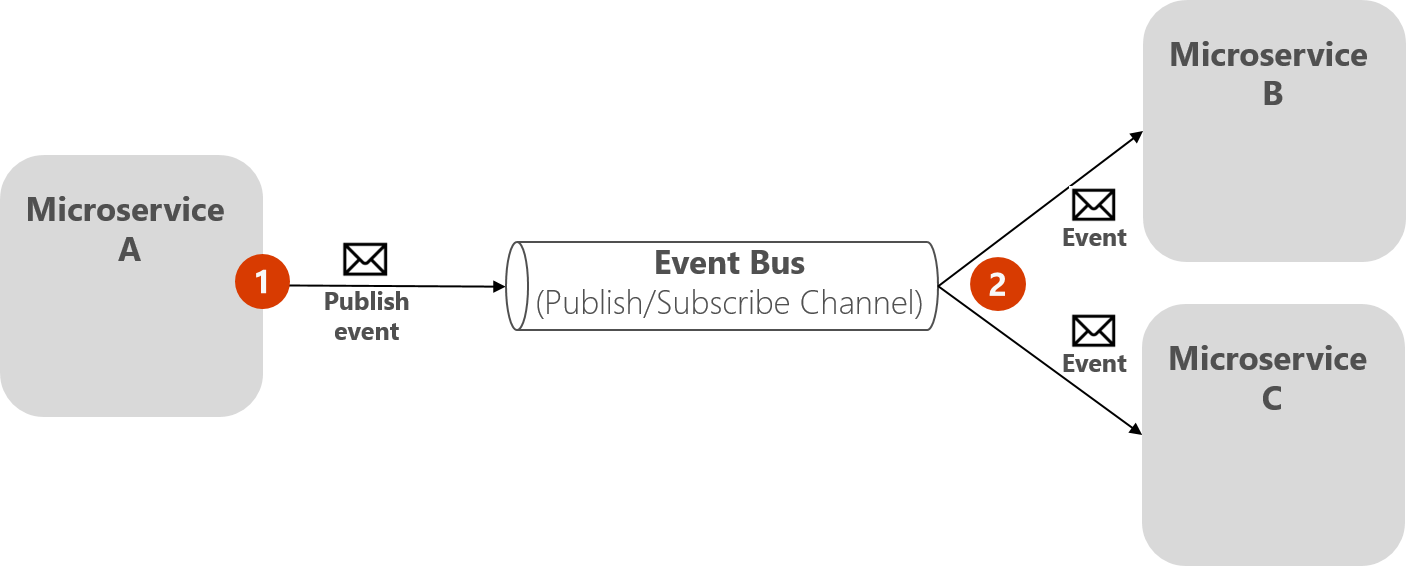
\includegraphics[width=0.5\textwidth]{microservices_bus}
	\caption[Eventbus mit Events] { Eventbus mit Events\cite{cesardelatorre2018azure}}
	\label{fig:microservices_bus}
\end{figure}

In dieser Abbildung haben Microservice B und C das Event x beim Ergeinisbus (\textbf{Event Bus}) abonniert (\textbf{subscribed}). D.h. Microservice A veröffentlicht (\textbf{published}) eine Änderung, woraufhin B und C informiert werden. B und C können nun ihren Datenbestand aktualisieren und halten so die aktuellen Daten vor. Parallel kann der Microservice A seine Abfrage ganz normal weiterführen. Der Eventbus ist dementsprechend ein Vermittler (\textbf{Message Broker}), welcher garantiert, dass die Nachrichten übertragen werden. Dieser sollte mit etwaigen Fehlerfällen (z.B. C ist nicht erreichbar) umgehen können und eine spätere Übertragung garantieren.\cite{cesardelatorre2018azure}\cite{wolff2018mic_praxis} \\

Aus diesem Modell ergibt sich ein weiterer Vorteil: Die Microservices sind entkoppelt. Es wird keine REST-Schnittstelle definiert, welche eine gewissen Fachlogik vorgibt. Ebenfalls können mehrere Services auf ein Event hören. Wolff warnt allerdings davor Events unnötig aufgebläht zu gestalten: Zum einen werden schnell Daten übermittelt, die nicht für alle Abonnenten (\textbf{Subscriber}) relevant sind und zum anderen entspräche dies nicht dem Prinzip vom DDD.\cite{wolff2018mic_praxis} \\

% Verhindern, dass Message Broker nicht erreichbar ist, durch
% - Der Message Broker sollte redundant laufen, wodurch schonmal eine hohe Wahrscheinlichkeit existiert, dass er erreichbar ist
% - Häufig ist es bei den Systemen so, dass man bspw. Innerhalb einer DB Transaktion in eine Tabelle schreibt, welche Events an den Broker dispatcht werden sollen. Und dann gibt es einen Background Task, der regelmäßig schaut, welche Events noch nicht an den Broker geliefert wurden und sendet die dahin
%- Wenn das fehlschlägt, dann versucht er es später wieder
%- Und das mit der Transaktion hat den Vorteil, dass eventuelle Änderungen in der DB garantiert  klappt oder beides (auch Speichern d. Events in einer Dispatcher Tabelle) fehlschlägt. Aber keine Inkonsistenzen

Zusätzlich sollte beachtet werden, dass Microservices so gestaltet werden, dass sie idempotent sind. In diesem Zusammenhang bedeutet dies, dass falls ein selbes Event zweimal übertragen wird, der Microservice die Aktion nicht zweimal ausführt. D.h. eine Mehrfachausführung führt zu demselben Ergebnis wie eine einzige Ausführung. Wenn z.B. eine Rechnung versendet werden soll, ist garantiert, dass diese nur ein einziges Mal versendet wird.\cite{wolff2018mic_praxis} \\

\subsubsection{Abwägung asynchrone vs. synchrone Kommunikation}

Aus den zwei vorherigen Abschnitten ergibt sich folgende Aufstellung (siehe Tabelle \ref{tab:sync_vs_async_table}).

\begin{table}[H]
	\begin{center}
		\begin{tabular}{|p{1,5cm}|p{5cm}|p{5cm}|}
			& synchrone Kommunikation & asynchrone Kommunikation \\ \hline
			 Vorteile
			&
				\begin{itemize}
					\item Jederzeit konsistent
					\item Paradigma ist Entwicklern bekannt\cite{wolff2018mic_praxis}
				\end{itemize} 
			& 
				\begin{itemize}
					\item Entkoppelt durch Events 
					\item Flexibilität, da ein Event mehre Services erreichen kann
					\item Nachrichtenempfang garantiert (ggf. mit Verzögerung)
					\item Absicherung gegen Ausfall
				\end{itemize} 
  			\\ \hline
			Nachteile
		  &
 			  	\begin{itemize}
				 	\item Anfälligkeit durch Abhängigkeiten 
				 	\item Erweiterbarkeit ist schwerer, da fachliche Abhängigkeiten
				 	\item Ggf. lange Netzwerkzeiten
				 \end{itemize}
		  & 
		 	\begin{itemize}
		 		\item nicht jederzeit garantiert konsistent
		 		\item Idempotenz muss beachtet werden
	 		\end{itemize}  \\ \hline
		\end{tabular}
	\end{center}
	\caption[synchrone vs. asynchrone Kommunikation]{synchrone vs. asynchrone Kommunikation}
	\label{tab:sync_vs_async_table} 
\end{table}

Es lässt sich feststellen, dass die Vorteile einer asynchronen Kommunikation für Microservices überwiegen, weshalb diese Kommunikationsart auch empfohlen wird.\cite{wolff2018mic_praxis}\cite{bruce2019mic_in_action} Dennoch ist die Kommunikation nicht dogmatisch zu betrachten, sondern sollte je nach Projekt und Anwendungsfall entschieden werden. Synchrone Kommunikation bietet sich nämlich gerade dann an, wenn der Datenbestand definitiv konsistent sein soll. \\

Das sogenannte CAP-Theoreom beschreibt die Abwägung, welche man in verteilten Systemen bei der Auswahl der Kommunikation tätigen muss. CAP bedeutet:
	\begin{itemize}
		\item Consistency (Konsistenz): Die Daten in einem verteilten System sind konsistent.
		\item Availability (Verfügbarkeit): Die Verfügbarkeit für alle Systeme ist gegeben. 
		\item Partition Tolerance (Partitionstoleranz): Das Gesamtsystem arbeitet auch weiter, wenn Teile davon ausfallen. 
	\end{itemize}  

In einem verteilten System können immer nur zwei von den drei Bedingungen erfüllt sein.\cite{wolff2018mic_praxis} Sofern Konsistenz gewährleistet werden soll, müssen alle Dienste stets verfügbar sein. Damit kann der Punkt Partitionstoleranz nicht mehr erfüllt sein. Umgekehrt: Wenn die Partitionstoleranz garantiert ist, z.B. dadurch dass Services ihre eigene Datenhaltung besitzen, ist zwar prinzipiell auch die Verfügbarkeit gegeben, aber nicht die Konsistenz. \\

Dementsprechend ist es sinnvoll, sich die System-Anforderungen zu überlegen und aufgrund dieser Basis zu entscheiden, welche Kommunikationsart implementiert werden soll. 

\subsubsection{API Gateway}

Umso mehr Services aufgesetzt werden, desto komplexer ist es, die Übersicht über alle zu behalten. Eine Abhilfe im Routing bietet ein sogenanntes \textit{API Gateway}. Ein API Gateway ist der einzige Einstiegspunkt für den Nutzer (\textbf{Client}). Von dort wird er weitergeleitet, ohne die Routen von einzelnen Services zu kennen. 

\begin{figure}[ht]
	\centering
	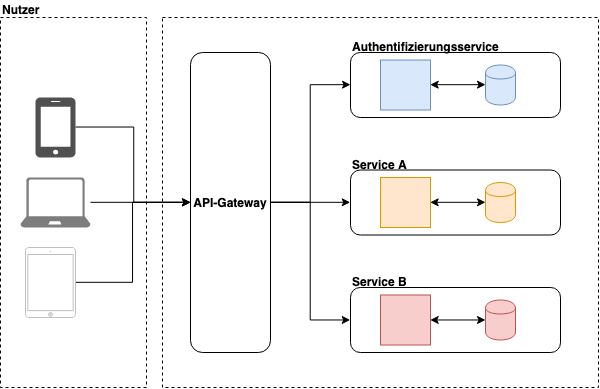
\includegraphics[width=0.6\textwidth]{api_gateway}
	\caption[Prinzip API Gateway] { Prinzip API Gateway }
	\label{fig:api_gateway}
\end{figure}

Abbildung \ref{fig:api_gateway} zeigt deutlich, wie die Nutzer über das API Gateway anfragen, welches anschließend an die entsprechenden Services weiterleitet. Wenn APIs eine hohe Auslastung haben, würde man mehrere Instanzen von einem API Gateway erstellen. Ein sogenannter Load Balancer wäre der Einstiegspunkt für die Clients. Dieser würde die Anfragen sinnvoll an die API Gateway Instanzen verteilen, so dass keine Überlastung entsteht.\cite{oracle} \\

API Gateways haben neben dem einzelnen Einstiegspunkt noch weitere Vorteile: 
\begin{itemize}
	\item Höhere Sicherheit darüber, dass einzelne Services nicht sichtbar und nur über das Gateway zu erreichen sind.\cite{bruce2019mic_in_action}
	\item Authentifizierung kann bereits im Gateway ausgeführt werden, dies führt zu weniger Last für einzelne Microservices.\cite{wolff2018mic_praxis}
	\item Zentralisiertes Logging, Caching, Monitoring, Mocking sowie eine zentralisierte Dokumentation ist möglich.\cite{wolff2018mic_praxis}
\end{itemize}  

Ein Nachtteil in der Struktur des API-Gateways ist, dass die Abfragen länger sind, da sie immer erst über das Gateway gehen.\\

\subsection{Authentifizierung und Autorisierung}\label{sec:authentifizierung_autorisierung}

Beim Monolithen ist architektonisch klar, dass die Authentifizierung und Autorisierung innerhalb des Monolithen stattfindet. Im Bereich der Microservice-Architektur existieren verschiedene Szenarien, wie man eine Authentifizierung sowie Autorisierung gestalten kann.\cite{bruce2019mic_in_action} \\

\textbf{Authentifizierung}: Identifiziert, wer jemand ist. Z.B. Nutzer A, der sich durch Benutzername und Passwort registriert hat.\cite{bruce2019mic_in_action}\\

\textbf{Autorisierung}: Bestimmt, wie viel ein Nutzer darf. Nutzer A hat eine Rolle, welche ihn berechtigt, gewisse Aktionen durchzuführen.\cite{bruce2019mic_in_action}\\

Wenn möglich und sinnvoll, kann die Autorisierung auch bereits im Gateway geschehen. Häufig muss allerdings ein Microservice diese selbst durchführen. Teils ist dies begründbar durch den Datenbestand, welcher nur dem Microservice vorliegt. \\

Um unnötige Last zu verhindern, kann die Validität (handelt es sich um einen gültigen Request) und die Authentifizierung bereits im API Gateway überprüft werden. Der weitere Vorteil ist, dass die Authentifizierung somit an einer zentralen Stelle durchgeführt wird. Dies verhindert Redundanz und fehlerhafte Implementierungen.\cite{rewe2019mic_ppp}\cite{richardson2019mic_pattern} \\

Die Idee ist, dass der Benutzer nach dem Anmelden ein Security-Token erhält, welches verwendet wird, um sensible Anfragen zu verifizieren. Zum einen gibt es die Möglichkeit, ein Token auszustellen, welches beim Auslesen verschlüsselt ist (opaque Token) und zum anderen auf einen offenen Standard namens \textit{JSON Web Token} (JWT, transparent Token) zu setzen. Das opaque Token hat den großen Nachteil, dass es zusätzliche Performance sowie Latenz verursacht und nur synchron entschlüsselt werden kann.\cite{richardson2019mic_pattern} \\

Das JWT wird beim Ausstellen signiert, um die Echtheit zu gewährleisten. Während die Nachteile des opaque Tokens hier nicht auftreten, ist ein anderes Problem, dass ein JWT nach Ausstellung nicht widerrufen werden kann. Theoretisch wäre es dauerhaft gültig, weshalb Ablauflaufzeiten gesetzt werden. Dies wiederum impliziert, dass der Client dafür sorgen muss, immer rechtzeitig ein neues Token anzuforden. Für solche und weitere Logiken exisitiert bereits ein Sicherheitsstandard namens OAuth2, welcher empfohlen wird zu verwenden.\cite{richardson2019mic_pattern} \\

Ziel bei OAuth2 ist unter anderem, Autorisierungen zwischen verschiedenen Anwendungen zu erlauben. Ursprünglich wurde das Authentifizierungsprotokoll so entworfen, dass Drittanwendungen Zugang zu Informationen erhalten, ohne dass Passwörter weitergeleitet werden müssen.\cite{richardson2019mic_pattern}  Beispielsweise wird OAuth2 verwendet, wenn Benutzer sich über ihren Facebook-Account bei Drittplattformen anmelden. Die Drittplattformen können natürlich nicht das Facebook-Passwort einsehen, erhalten aber je nach Anwendungsfall Zugriff auf verschiedene Ressourcen (z.B. Lesezugriff auf die E-Mail-Adresse und/oder Konakte, Schreibzugriffe zum Teilen von Nachrichten usw.). \\

Da OAuth2 ein sehr komplexes und umfangreiches Thema ist, wird im Folgenden nur ein häufig verwendetes Grundprinzip erklärt. \\

Um die Abbildung \ref{fig:password_grant} besser zu verstehen, sind folgende Definitionen hilfreich:\cite{richardson2019mic_pattern}\\

\textbf{Authorization Server}: Authentifiziert den Benutzer und gibt ein Access sowie Refresh Token raus.\\

\textbf{Access Token}: Durch ein Access Token erhält man Zugriff auf den Resource Server. Das Format ist abhängig von der jeweiligen Implementierung, eine bereits genannte Möglichkeit wäre JWT. Der Access Token ist zeitlich begrenzt gültig. \\

\textbf{Refresh Token}: Ein Token, welches langlebig ist, also eine lange Gültigkeit besitzt. Dieses kann allerdings im Gegensatz zum Access Token widerrufen werden. Ebenfalls wird es verwendet, um ein neues Access Token vom Authorization Server anzufordern. Dafür ist keine Übergabe der Benutzerdaten nötig.\\ 

\textbf{Resource Server}: Eine Ressource auf die nur zugegriffen werden kann, wenn ein valides Access Token vorliegt. Eine Ressource könnte z.B. ein Microservice sein.\\ 

\textbf{Client}: Ein Client möchte Zugriff auf den Resource Server. Clients können beispielsweise Drittanwendungen, Webanwendungen oder mobile Applikationen sein. Sie werden auch Resource Owner genannt. \\ 

\begin{figure}[H]
	\centering
	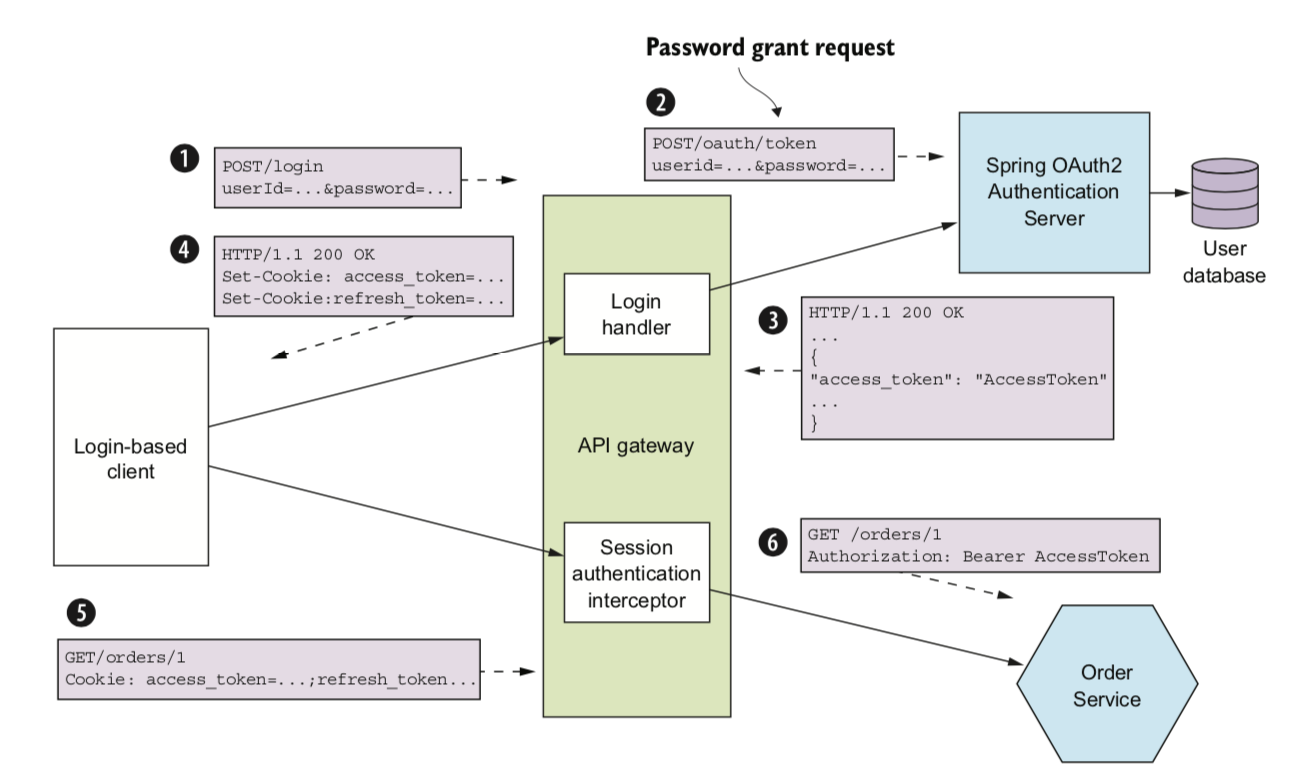
\includegraphics[width=0.7\textwidth]{password_grant}
	\caption[Ablauf eines password grants] { Ablauf eines sogenannten `password grant`\cite{richardson2019mic_pattern} }
	\label{fig:password_grant}
\end{figure}

Die Abbildung \ref{fig:password_grant} zeigt einen Ablauf, bei dem ein Client seinen Usernamen und sein Passwort übermittelt (1). Diese Anfrage wird von dem API Gateway weitergeleitet an einen Authorization Server (2). Wurde der Nutzer gefunden, wird ein Access und Refresh Token über das API Gateway (3) an den Nutzer übermittelt (4). Mit der entsprechenden Autorisierung ruft der Client seine Bestellungen (5) ab. Dieser Request wird entsprechend von dem API Gateway weitergeleitet (6). \\

Neben dem \textit{password grant Flow} existiert auch der sogenannte \textit{client credentials grant Flow}. Dieser funktioniert ähnlich, nur dass nicht Username und Passwort übertragen werden, sondern geheime Daten für die Authentifikation zwischen Anwendung und Authorization Server bekannt sind. Den \textit{client credentials grant Flow} sollte man verwenden, wenn eine Applikation Ressourcen aufrufen möchte, die außerhalb eines User-Kontextes liegen, d.h. es handelt sich in der Regel um recht allgemeine Daten.\cite{oauth2}\cite{richardson2019mic_pattern} \\

Auf Basis dieses Abschnittes \ref{sec:authentifizierung_autorisierung} wird herausgearbeitet, welche Möglichkeiten zur technischen Umsetzung von OAuth2 bereitstehen (siehe \ref{sec:concept_authentifizierung_autorisierung}). 

\subsection{Docker}

Über Docker können Anwendungen innerhalb eines Containers laufen. Ein Container ist vergleichbar mit einer sehr leichtgewichtigen, modularen virtuellen Maschine.\cite{RedHat} Docker in der Tiefe aufzuarbeiten, würde den Umfang dieser Arbeit übersteigen. Dennoch wird im Folgenden erläutert, warum speziell Docker sich sehr gut für Microservices eignet und wie das grundsätzliche Wirkungsprinzip funktioniert. \\

Anfangs wurden Microservices so definiert, dass sie als möglichst eigenständige, deploybare Einheiten zu betrachten sind. Beim Hosten - also dem Bereitstellen des Services - sollte dies ebenfalls berücksichtigt werden. Nimmt man an, man hostet alle Services auf einer Maschine, läuft man Gefahr, dass die Microservices sich z. B. durch Portkonfigurationen oder dem Zugriff auf selben Ressourcen behindern.\cite{wolff2016mic_architectures} \\

Als bisherige Lösung boten sich an dieser Stelle virtuelle Maschinen (\textbf{VM}) an. D.h. auf einem Host könnten mehrere Betriebssysteme laufen, die sich die Hardwareressourcen vom Host teilen. Die angestrebte Isolation zwischen den Microservices wäre erreicht und individuelle Konfigurationsmöglichkeiten könnten sich gegensetitig nicht mehr stören. Durch die VMs entstehen allerdings Leistungseinbußen, welche nicht im Verhältnis zum Nutzen stehen und zusätzlich einen höheren Verbrauch der Hardwareressourcen mit sich bringen.\cite{wolff2016mic_architectures} Gesucht ist dementsprechend eine Technologie, die es schafft, Services zu isolieren und dabei gleichzeitig leichtgewichtig zu sein: Docker. \\

Startet man einen Microservice über Docker, ist dies damit gleichzusetzen, als würde im Betriebssystem der Service als Prozess gestartet werden. Es entsteht kein deutlich sichtbarer Overhead in Bezug auf den Ressourcenverbrauch.\cite{wolff2016mic_architectures} \\

Um den Docker-Aufbau (siehe Abbildung \ref{fig:docker_architektur_edited}) besser zu verstehen, ist folgendes Vokabular nützlich:\cite{wolff2016mic_architectures} \\

\textbf{Docker-Image}: Aus einer Anwendung kann man ein Image erzeugen, so dass es im Docker-Container gestartet werden kann.  \\

\textbf{Docker-Container}: Wenn ein Image ausgeführt wird, läuft es in einem Container, welcher verschiedene Eigenschaften hat, wie z.B. ein eigenes Netzwerk-Interface und ein Dateisystem.\\

\textbf{Dockerfile}: Ein Dockerfile ist ähnlich einem Bauplan. Er beschreibt, wie das Image gebaut werden muss, damit es in einem Docker-Container laufen kann. \\

\textbf{Repository}: Ein Repository speichert Images. In der Regel hält ein Repository mehrere Images von derselben Anwendung mit verschiedenen Versionen bereit.\cite{RedHat} \\

\textbf{Docker-Registry}: Eine Docker-Registry verwaltet mehrere Repositories. \\

\textbf{Docker-Host}: Ein Docker-Host unterstützt die Docker-Technologie, d.h. es können entsprechend Images ausgeführt werden. Zusätzlich ist es möglich, Images von einem Repository auszuführen. D.h. man muss die Images nicht extra auf den Host laden, um sie auszuführen. \\

Bei genauerer Betrachtung der Abbildung \ref{fig:docker_architektur_edited} fällt auf, dass Container in einem Netzwerk sind und sich denselben Kernel teilen. Dateisysteme, Netzwerk-Interface und containereigene Prozesse sind voneinander isoliert. D.h. Portfreigaben oder ähnliche Konfigurationen behindern sich nicht. \\

\begin{figure}[H]
	\centering
	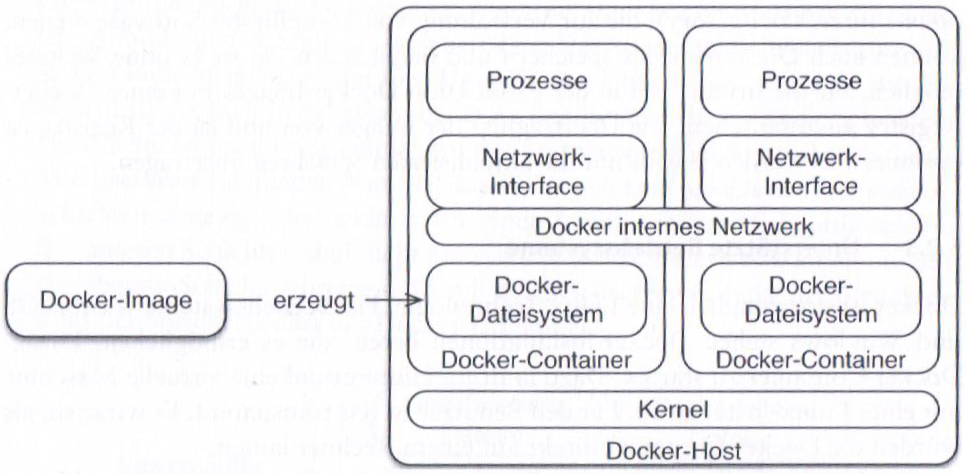
\includegraphics[width=0.7\textwidth]{docker_architektur_edited}
	\caption[Docker Architektur] { Docker Architektur\cite{wolff2016mic_architectures} }
	\label{fig:docker_architektur_edited}
\end{figure}

Zusammenfassend lässt sich sagen, dass sich durch das Nutzen von Docker eine isolierte und ressourcenvertretbare Trennung von Microservices auf einem Host erreichen lässt. \\


\section{Konzept}
Das ist die Konzepteinleitung

\subsection{Anforderungen definieren}
Um die Anforderungen für das Spiel \textit{Stirnraten} zu erfassen, sollten zwei verschiedene Aspekte berücksichtigt werden: 

\begin{itemize}
	\item der \textbf{IST-Stand}, was muss mindestens erfüllt werden und 
	\item welche möglichen \textbf{Erweiterungen} entstehen durch eine API.
\end{itemize}

Um die Anforderungen greifbarer zu gestalten, wird auf das Prinzip von User Story Mapping zurückgegriffen. D.h. jede Anforderung ergibt sich aus einer sogenannte User Story. Diese ist so aufgebaut, dass beschrieben wird \textbf{wer} möchte \textbf{was} und \textbf{aus welchem Grund}.\cite{UserStoryMapping}\\

Im Folgenden gelten die zwei Definitionen: Ein Nutzer ist eine Person, welche die App spielt. Der Betreiber ist der Besitzer von Stirnraten. Ein User kann ein Nutzer oder Betreiber sein. \\

Ein Beispiel für eine User Story könnte lauten: Als Nutzer (\textit{wer}) möchte ich mein Spielprofil teilen (\textbf{was}), um mich besser mit meinen Freunden messen zu können ({\textbf{warum}).\\
	
Wie diese User Story nun umgesetzt wird, muss abgewogen werden. Zum einen sollten User Stories konkret genug formuliert werden, so dass klar ist, was der User möchte. Zum anderen bleibt bei der Entwicklung ein agiler Handlungsspielraum.\cite{UserStoryMapping} Eine Teile-Funkion beispielweise kann unterschiedlich aufwendig umgesetzt werden. Der Nutzer könnte ein Text teilen, ein extra aufbereitets Bild oder einen Link, welcher auf ein mögliches Online-Profile verweist. All diese Möglichkeiten bedeuten unterschiedliche Aufwände. Alternativ könnte man aus dieser einen User Story drei erstellen, welche entsprechend unterschiedlich priorisiert werden.\\

\textit{Exkurs - Spielprinzip Stirnraten: Die Spieleranzahl muss mindestens zwei betragen. Ein Spieler wählt aus verschiedenen Kategorien aus und hält sich das Telefon an die Stirn. Es erscheint Begriff, welchen der Gegenüber erklären muss. Errät der Spieler den Begriff, neigt er das Telefon nach vorne und ein neuer Begriff erscheint. Weiß er ihn nicht, kann er diesen überspringen, in dem er das Telefon nach hinten neigt. Ziel ist es, innerhalb einer frei wählbaren Zeit (z.B. 60 Sekunden), so viele Begriffe wie möglich zu erraten.}

\subsubsection{Erfassung Stirnratens IST-Stand}

In der folgenden Tabelle \ref{tab:bestehende_funktionen} wird gezeigt, welche Funktionen die App bereits auf dem Gerät bereitstellt, welche aber zukünftig serverseitig erledigt werden sollen. 

\begin{table}[H]
	\begin{center}
		\begin{tabular}{p{3cm}p{10cm}}
			Funktion & Beschreibung \\ \hline
			Profil/Statistik & Nach jedem Spiel werden verschiedene Daten erfasst, z.B. die Dauer des Spiels oder richtig geratene Wörter. Löscht man die App, ist dieses Profil unwiederbringlich. \\
			Bereitstellung Begriffe & Die über 6000 verschiedenen Begriffe liegen nur offline zur Verfügung. Editieren, Hinzufügen und Löschen geht nur über das Updaten der App.\\
			Zweisprachigkeit & Die App wird für den deutschen sowie den englischen Sprachraum angeboten. Es ist gewährleistet, dass je nach Nutzer, auf die sprachlich richtige Datenbank zugegriffen wird.\\
		\end{tabular}
	\end{center}
	\caption[bestehende Funktionen in Stirnraten]{bestehende Funktionen in Stirnraten}
	\label{tab:bestehende_funktionen} 
\end{table}

Aus dem IST-Zustand ergeben sich bereits folgende User Stories: 

\begin{itemize}
	\item Als Betreiber möchte ich neue Begriffe über eine Schnittstelle hinzufügen, editieren und löschen können, um die Datenbank schneller und leichter zu pflegen
	\item Als Betreiber möchte ich eine Datenbank, um nicht für zwei Apps (iOS und Android) den Datenbestand zu pflegen
	\item Als Betreiber möchte ich entscheiden können, in welcher Sprache (englisch oder deutsch) ich Begriffe manipuliere, um sinnvolle Daten zu gewährleisten
	\item Als Nutzer möchte ich das Spiel immer offline spielen können, da ich auf Reisen häufiger kein stabiles Internet habe
	\item Als Nutzer möchte ich mein Spielerprofil online speichern, um es auf anderen Geräten oder nach einer Neuinstallation abrufen zu können
	\item Als Nutzer möchte ich automatisch die Sprache angezeigt kriegen, welche für mich relevant ist, weil es mir sonst zu kompliziert ist
\end{itemize}

\subsubsection{Erweiterungen mittels User Story Mapping}

Durch das Einführen einer API bieten sich folgende Erweiterungsmöglichkeiten an:

\begin{itemize}
	\item Als Betreiber möchte ich neue Kategorien hinzufügen, editieren und löschen können, um das Nutzerangebot zu vergrößern
	\item Als Betreiber möchte ich Bilder pro Kategorie hinzufügen, editieren und löschen können, um ein sprechendes Bild für die Nutzer zu hinterlegen
	\item Als Betreiber möchte ich eine Kategorie als Premium kennzeichnen können, um Angebotsaktionen zu schalten
	\item Als Betreiber möchte ich eine Kategorie (de)aktivieren können, um sie immer zu einem sinnvollen Zeitpunkt anbieten zu können
	\item Als Betreiber möchte ich eine Registrierfunktion anbieten, um die Nutzer stärker an mich zu binden.
	\item Als Betreiber möchte ich die Nutzer abrufen, welche sich bei mir registriert haben, um einen Nutzerstamm aufzubauen
	\item Als Betreiber möchte ich Nutzer aus Datenschutzgründen löschen können
	\item Als Nutzer möchte ich mich in einer Rangliste mit anderen Nutzern vergleichen können, um zu sehen, wer in dem Spiel besser ist.
	\item Als Nutzer möchte ich die Spielerprofile von anderen Nutzern detailliert ansehen, um zu sehen, was ihnen gefällt 
	\item Als Betreiber möchte ich die Ranglisten-Namen der Nutzer manipulieren können, um unflätige Namen/Missbrauch zu verhindern.
	\item Als Betreiber möchte ich kummulitierte Daten aus den Nutzerstatistiken sehen, um Marktentscheidungen besser treffen zu können
	\item Als Betreiber möchte ich die Kategorien sortieren können, um die Anordnung für die Nutzer bestmöglich zu gestalten
	\item Als Betreiber möchte ich sehen, wenn ein Begriff bereits in der Kategorie ist, um die Datenqualität zu gewährleisten
	\item Als Nutzer möchte ich eigene Begriffe einreichen können, weil mir manche Begriffe oder Kategorien im Spiel fehlen
	\item Als Nutzer möchte ich sehen, wenn ein eingereichter Begriff bereits in einer Kategorie existiert, um Bescheid zu wissen
	\item Als Betreiber möchte ich eingereichte Begriffe zulassen oder ablehnen können, um den Datenbestand zu vergrößeren bzw. die Qualität zu gewährleisten 
	\item Als Betreiber möchte ich sehen, wann meine Nutzer zuletzt online waren, um ggf. Marketingmaßnahmen zu unternehmen
	\item Als Betreiber möchte ich, dass Nutzer-Zugangsdaten entsprechend gut verschlüsselt sind, um die Datensicherheit zu gewährleisten
\end{itemize}

Die folgende Auflistung sind User Stories, welche auch als Anforderungen entstanden sind, aber im Rahmen der Projektarbeit aufgrund von Aufwänden nicht umgesetzt werden können.

\begin{itemize}
	\item Als Betreiber möchte ich eine Newsletter-Funktion anbieten, um die Nutzer über Neuigkeiten zu informieren
	\item Als Nutzer möchte ich ein Profilbild hochladen, um mein Profil zu indiviualisieren
	\item Als Nutzer möchte ich mein Passwort zurücksetzen können, wenn ich es vergessen habe. 
	\item Als Betreiber möchte ich individuelle Animationen vom Server an den Nutzer weiterreichen können, um die Verspieltheit der App zu unterstreichen.
	\item Als Betreiber möchte ich Themes und Farbcodes online bereitstellen, um den Nutzern Individualsierungsmöglichkeiten schneller und leichter bereitzustellen 
	\item Als Betreiber möchte ich automatisiert, individuelle (Push)Nachrichten senden, um den Nutzer stärker zu binden
\end{itemize}

Aus den User Stories ergeben sich konkrete Abhängigkeiten zwischen den Microservices sowie klare Vorlagen für die Datenhaltung, z.B. benötigt der Nutzer mindestens einen eindeutigen Namen sowie ein Passwort. Die konkrete Umsetzung ist in FIGURE-VERLINKEN-AUF-KAPITEL-5.

\subsection{Macroarchitektonische Festlegungen}
- MySQL, Docker, selbe Begründung
- REST (Verlinkung auf Mobile Development-Modul)
- Bounded Context erstellen 

\subsection{Wahl des API-Gateway}
- Ocelot 
- welches gibt es noch? 
- Eigenbau 

% Artikel lesen und Grundlagen rausarbeiten: https://docs.microsoft.com/de-de/dotnet/standard/microservices-architecture/secure-net-microservices-web-applications/

% Guter Artikel bzgl. OAuth2: https://medium.com/google-cloud/understanding-oauth2-and-building-a-basic-authorization-server-of-your-own-a-beginners-guide-cf7451a16f66

\subsection{Wahl der Kommunikation}
- Erwähnen, dass asynchrone Kommunikation verwendet wird, aufgrund der Vorteile aus den Grundlagen 
- Technologie: Masstransit (RabbitMQ) vs. Kafka

\subsection{Wahl der Authenfizierung/Authorisierung}
- Auth0
- OAuth2: Authentication Framework (mit OpenId Connect?) -> Spricht die Zeit, Komplexität und so eine Komplexität gar nicht benötigt 
- JWT: Also Protocol
- Dritteranbieter Dienst -> Auth0 (zu teuer)


\section{Implementierung}
Das ist der Implementierungspart

\section{Fazit}

Das Ziel, den Aufbau einer API basierend auf der Microservice Architektur anhand des Spieles Stirnraten, betrachte ich meiner Meinung nach als gelungen und abgeschlossen. Mittels Domain Driven Design konnten verschiedene Microservices detektiert und abgegrenzt werden. Unterstüzend diente User Story Mapping als Werkzeug zum Erfassen von Anforderungen. Diese wurden nach Priorität sortiert und es ist ein Produkt entstanden, welches aktiv eingesetzt werden kann. Ebenfalls werden weitere Ausbaustufen aufgezeigt, da selbstverständlich nicht  alle erfassten Anforderungen aus Kapazitätsgründen umgesetzt wurden. \\

Weiter wurde eine Microservice Architektur erschaffen, die den definierten Bewertungskriterien für Microservices entspricht. Zusätzlich wurden empfohlene Pattern wie das Verwenden eines Gateways und das Nutzen der asynchronen Kommunikation angewandt. Die Authentifizierung sowie Autorisierung bietet ein hohes Maß an Flexiblität. Dies bedeutet, dass weitere Microservices, aber auch etwaige Drittnutzer, einen kontrollierten Zugriff auf die API erhalten könnten.\\

Trotz der erfolgreichen Umsetzung, gilt darauf hinzuweisen, dass der Umfang der Anforderungen an dieses Projekt derzeit keine Microservice Architektur rechtfertigen würde und deshalb eher prototypisch zu betrachten ist. Durch die vielen verschiedenen Microservices ist Mehrarbeit entstanden. Beispielsweise hätte die Datenstruktur mühelos auf eine Datenbank abgebildet werden können, stattdessen wurden drei Datenbanken verwendet. 

%SERVICE MESH oder SERVICEMESH
\subsection{Ausblick}
Diese Projektarbeit bietet noch zahlreiche, technische Erweiterungen an. Die Portvergabe und das Zusammenspiel der Microservices war aufwändig und teilweise sehr fehleranfällig, da es manuell und per Hand betrieben worden ist. Wenn die Serviceanzahl wächst, ist dies tendenziell eine große Fehlerquelle, da es ein hoher Arbeitsaufwand ist, nicht den Überblick zu verlieren. Dafür gibt es bereits mögliche Lösungen. Zum einen wäre Kubernetes als Orchestrierungsprogramm möglich. Zum anderen könnte ein sogenannter Service-Mesh erforscht werden, bei dem die Microservices sehr vereinfacht ausgedrückt, sich selbst ins System einpflegen. \\

Zusätzlich sollte eine automatisierte Build- und Deploymentstruktur (CI/CD) erschaffen werden. Open Source Tools wie z.B. Jenkins oder kostenpflichtige Tools wie z.B. Bamboo bieten zahlreiche Automatisierungsoptionen. Automatisierte Build- und Deploymentscripts sparen viel Zeit und Aufwand. \\

Wenn die Last wächst, sollten Microservices skalierbar sein. Das Verwenden von mehreren Servern und einem Loadbalancer, der die Last entsprechend verteilt, wären mögliche Lösungsansätze. Natürlich müssen dabei zusätzliche Aspekte beachtet werden, wie z.B. dass keine Inkonsistenzen in den Datenbanken entstehen. \\

Der letzte und möglicherweise wichtigste Punkt ist, die Microservices zu überwachen. Dies umfasst, entstandene Errors zu erkennen (Logging). Dafür gibt es bereits etablierte Tools wie z.B. den ELK Stack (Elasticsearch, Logstash, Kibana). Ebenfalls sollten Strategien überlegt werden, was passiert, wenn ein Service ausfällt und wie man diesen Zustand bereits frühzeitig bemerkt (Health Check). \\
 
Natürlich sind die genannten Ausblicke auch für eine monolithische Anwendung wichtig, allerdings bewerte ich die Umsetzung der genannten Punkte in einer Microservice Architektur als komplexer und umfangreicher. Umso größer die Anwendung wird, desto eher sollte man eine Microservice Architektur verwenden.
\pagebreak

\printbibliography

